\documentclass{beamer}
\usepackage{multicol}
\usepackage{natbib} 
\def\newblock{\hskip .11em plus .33em minus .07em}
\newcommand\independent{\protect\mathpalette{\protect\independenT}{\perp}} 
\def\independenT#1#2{\mathrel{\rlap{$#1#2$}\mkern2mu{#1#2}}} 
%\usepackage{beamerthemeBerkeley}
% Use either the one above or the one below
\usetheme{Hannover}

\title{Regression Discontinuity}
%\author{	F. Daniel Hidalgo\\ }
%\date{\today}

\begin{document}

\frame{\titlepage}

%\section[Outline]{}
%\frame{\tableofcontents}

\section{Basic Setup}

\frame{
	\frametitle{Living on the Edge}
\begin{itemize}
	\item $T_i=1[X_i\geq c]$
        \item $\tau_{rd} = E[Y_i(1)-Y_i(0)|X_i=c]$
\end{itemize}
\textbf{Assumptions}
\begin{enumerate}
\item  $Y_i(0),Y_i(1) \independent T_i|X_i$
  \begin{itemize}
  \item This assumption is trivially met, because conditional on $X$,
    there is no variation left in $T$, so it cannot be correlated with
    unobservables. 
  \end{itemize}
\item $0 < \textrm{P}(T_i=1|X_i=x)<1$
  \begin{itemize}
  \item In the sharp regression design, this is \textit{always}
    violated. 
  \end{itemize}
\item $E[Y(0)|X=x]$ and $E[Y(1)|X=x]$ are continuous  in $x$.
  \begin{itemize}
  \item Continuity is required to compensate for the failure of the
    common support condition. 
  \end{itemize}
\item SUTVA
\end{enumerate}
}


\begin{frame}
  \frametitle{Probability of Treatment}
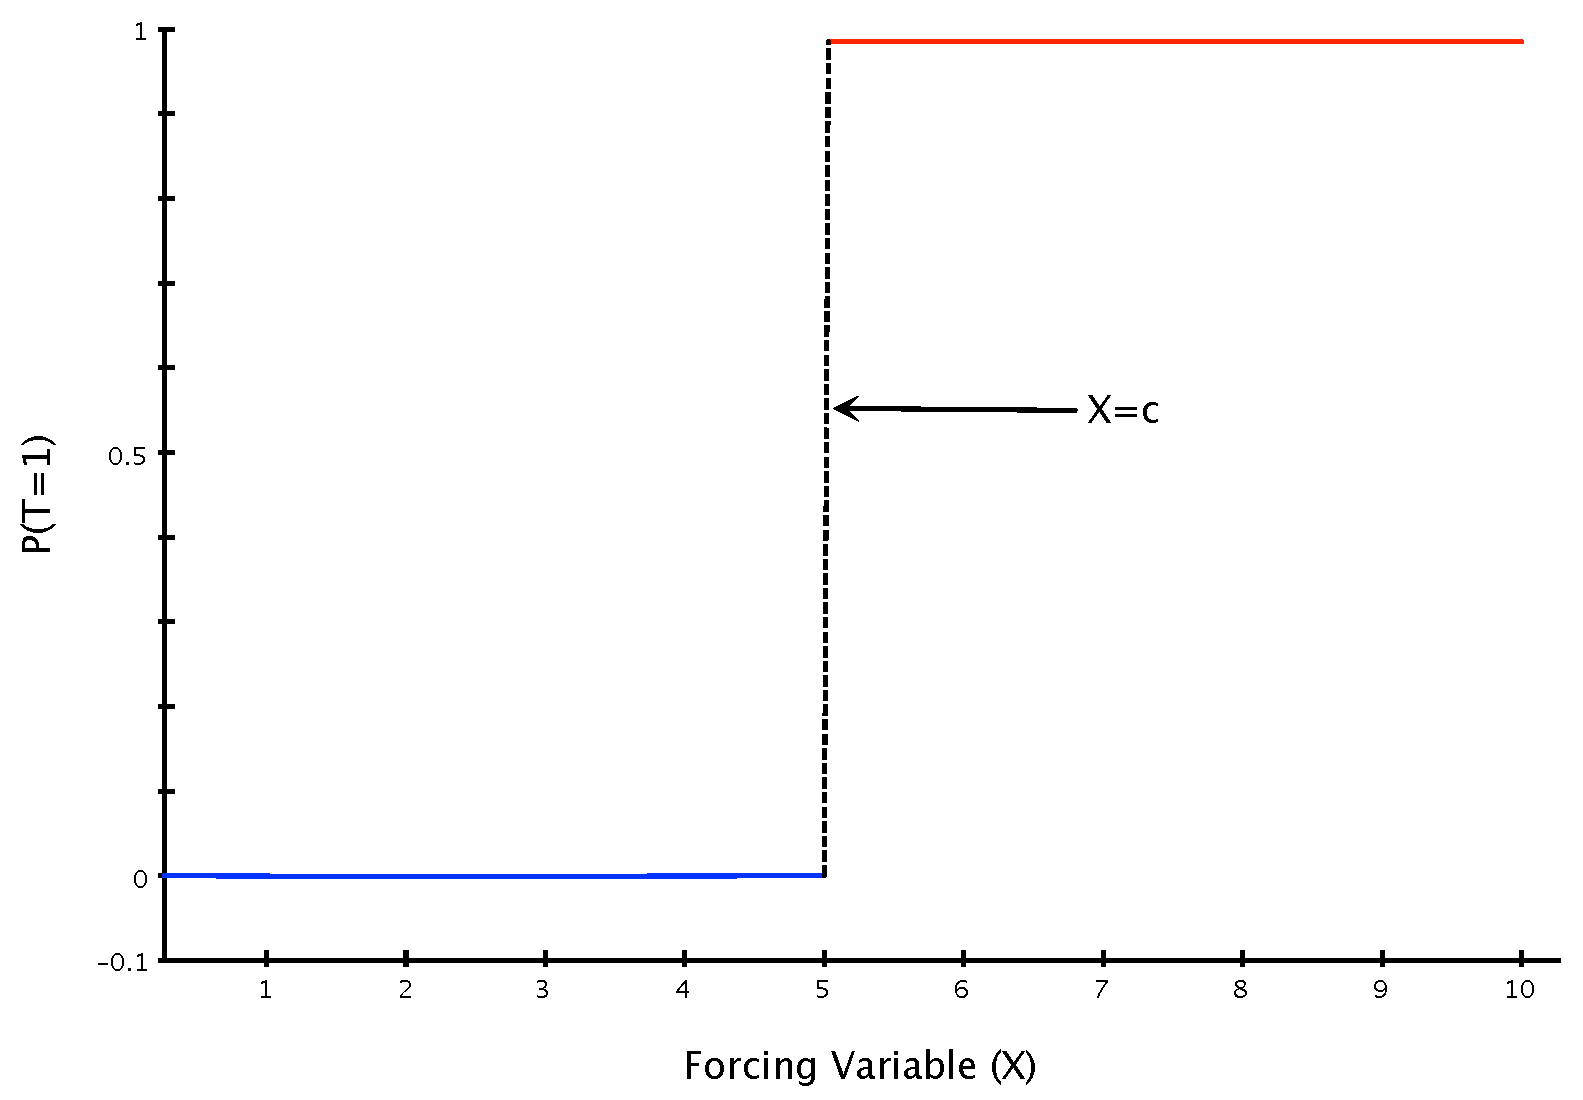
\includegraphics[width=9cm]{sharpRD_assign_prob.pdf}  
\end{frame}

\begin{frame}
  \frametitle{Simple Linear RD Setup}
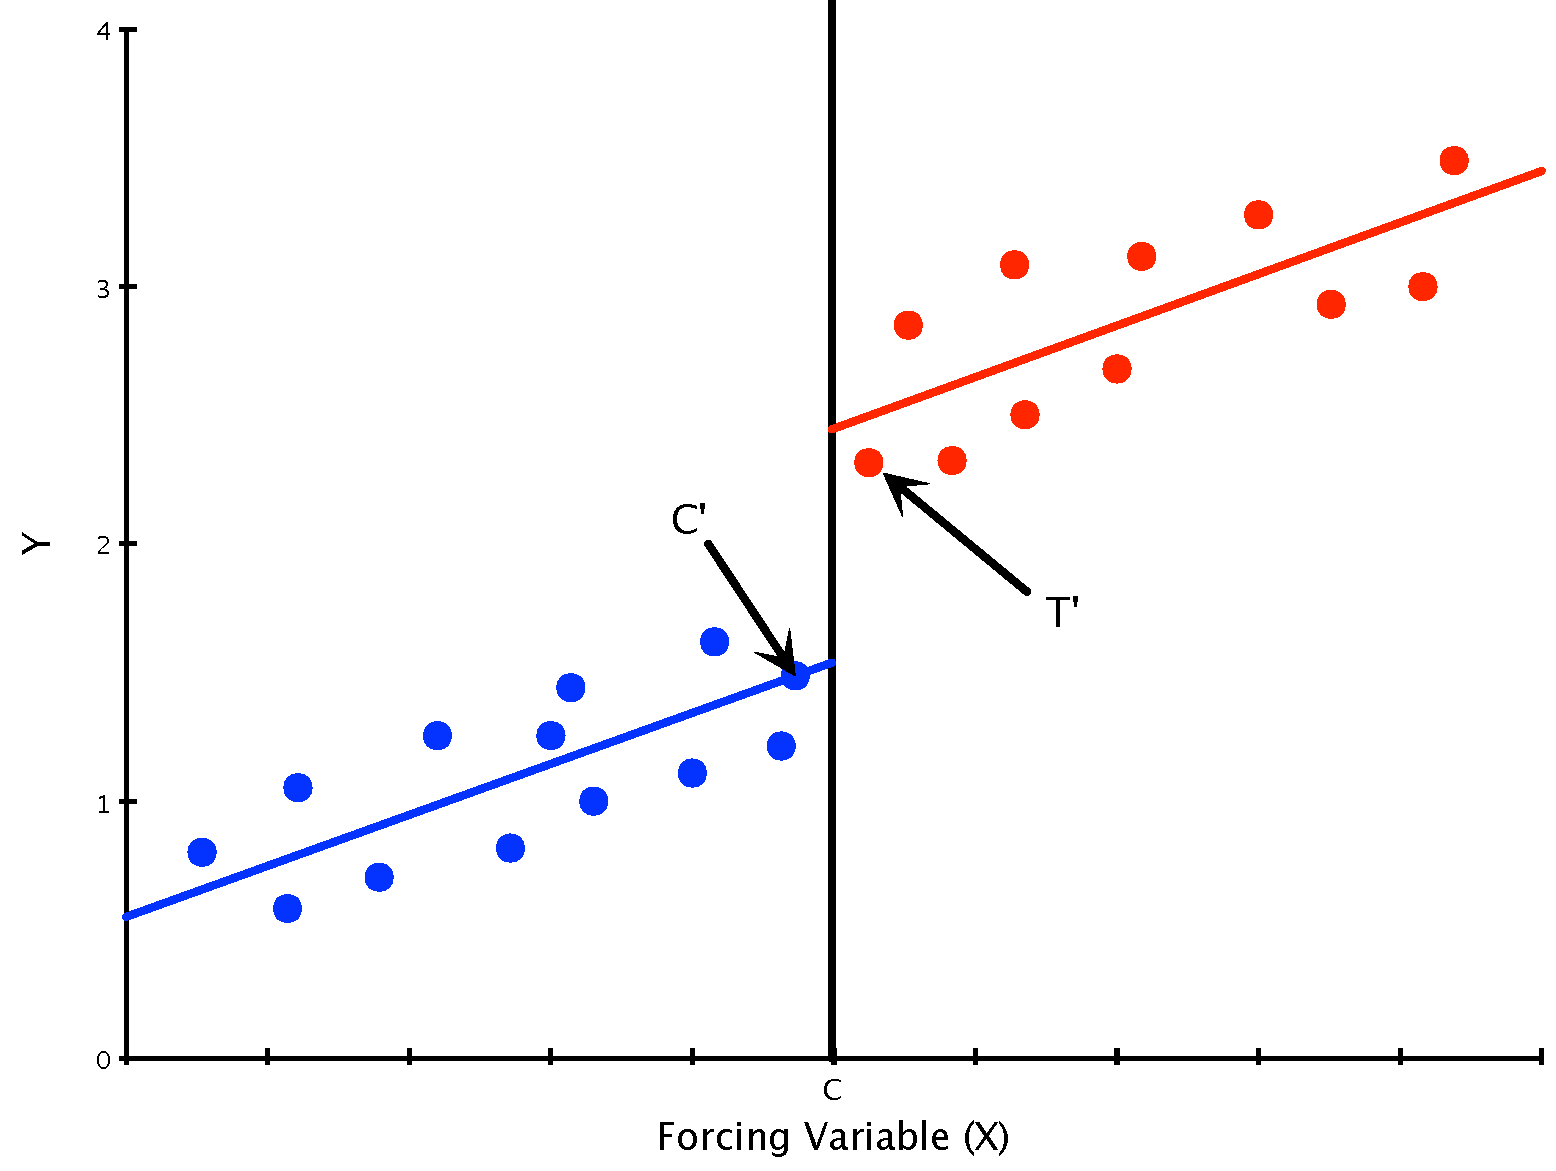
\includegraphics[width=9cm]{linear_reg_discont.pdf}  
\end{frame}


\begin{frame}
  \frametitle{Potential Outcomes}
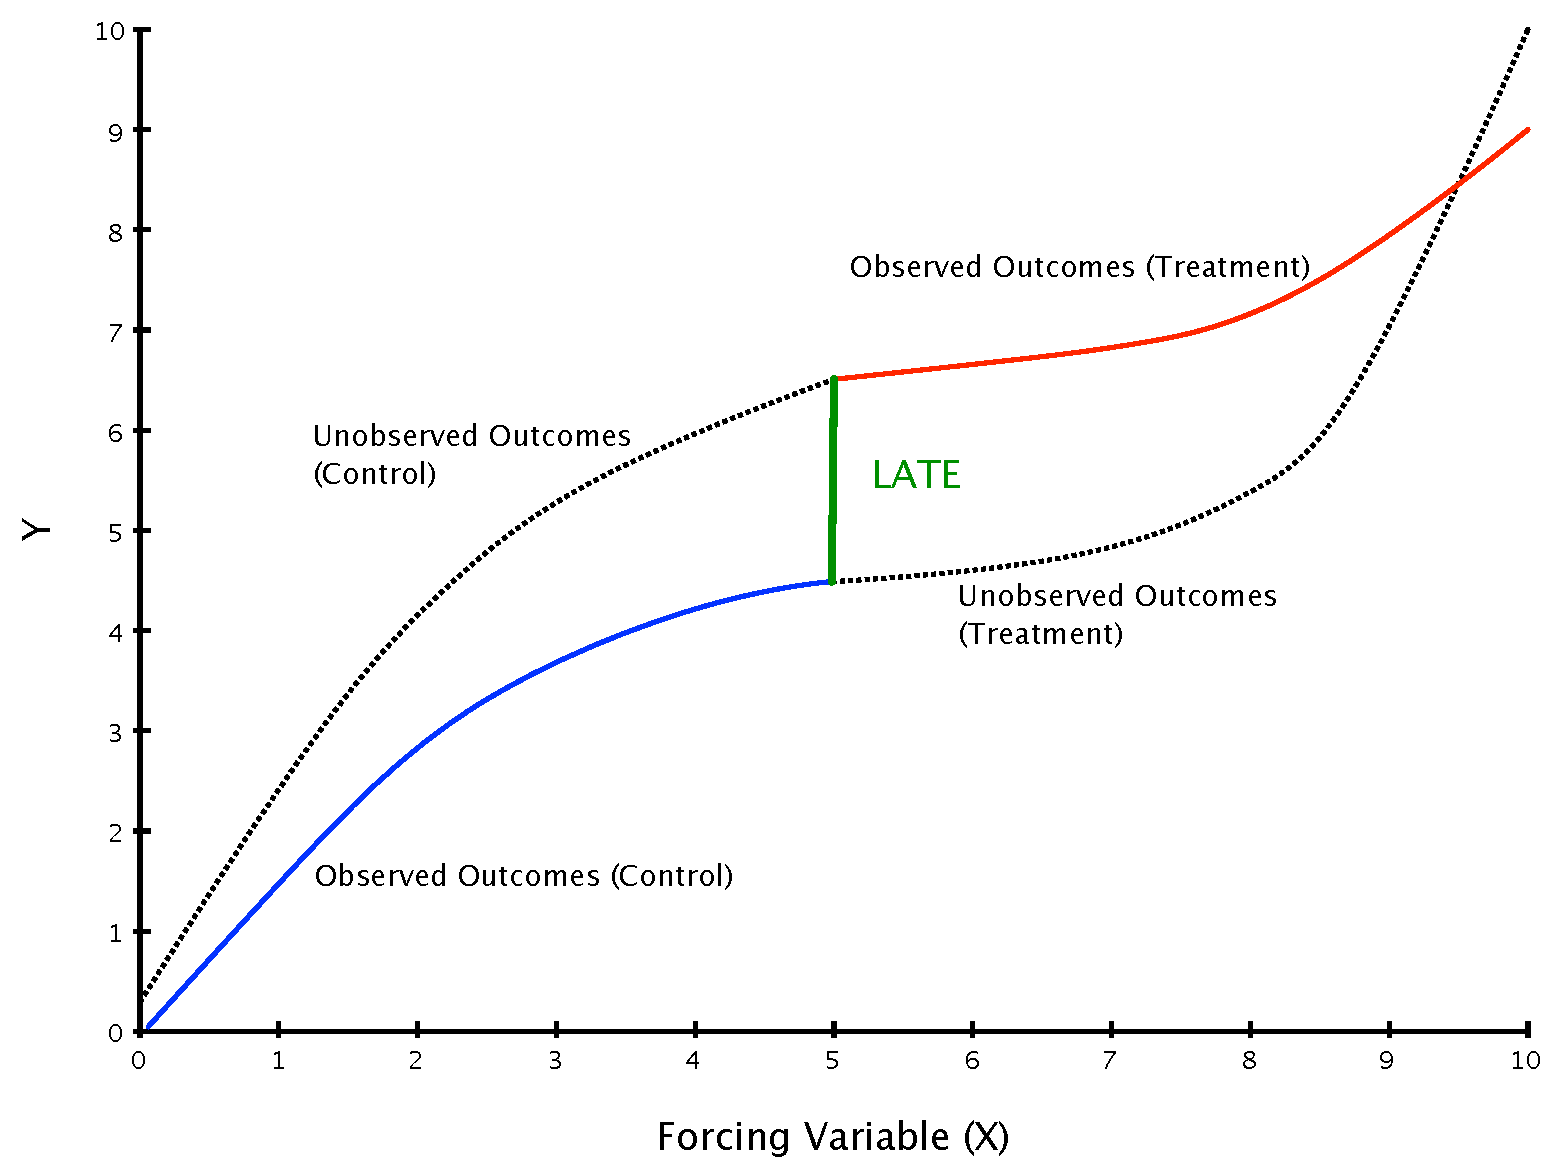
\includegraphics[width=9cm]{RD_potential_outcomes.pdf}  
\end{frame}

\section{Lee's Interpretation} % (fold)
\label{sec:lee_s_interpretation}

% section lee_s_interpretation (end)
\begin{frame}[c]\frametitle{Lee's Interpretation}
	\begin{itemize}
		\item<+-> Most important question: Are individuals able to influence the assignment variable, and if so, what is the nature of this control?
		\item<+-> 
		\begin{align*}
			Y =& D\tau + W\delta_1 + U\\
			D =&1[X\geq c] \\
			X =&W\delta_2 + V
		\end{align*}
		where $Y$ is outcome of interest, $D$ is the binary treatment indicator, $W$ is a vector of pre-treatment observable characteristics of the individual that might affect the outcome and/or assignment variable.
		\item<+-> $W$ is endogenously determined, $\delta_1$ and $\delta_2$ need not be 0, no assumptions about correlations between $W$, $U$, and $V$.
	\end{itemize}
\end{frame}

\begin{frame}[t]\frametitle{Lee's Interpretation}
	\begin{itemize}
		\item<+-> Heterogeneity in the outcome is completely described the pair of random variables ($W$, $U$)
		\item<+-> The distribution of $X$, conditional on a particular pair of values $W=w, U=u$, is equivalent (apart from an additive shift) to the distribution of $V$ conditional on $W=w, U=u$
		\item<+-> If there is some room for error, but individuals have precise control about whether they fail to receive the treatment, then the density of $X$ will be 0 below the threshold, but positive above the threshold. 
		\item<+-> If there is stochastic error in the assignment variable and individuals do \emph{not} have precise control over the assignment variable, we would expect the density of $X$ (and hence $V$), conditional on $W=w, U=u$ to be continuous at the discontinuity threshold. 
	\end{itemize}
\end{frame}

\begin{frame}
  \frametitle{Is our RD Design Valid?}
Are individuals able to influence the forcing variable, and if so,
what is the nature of this control?
  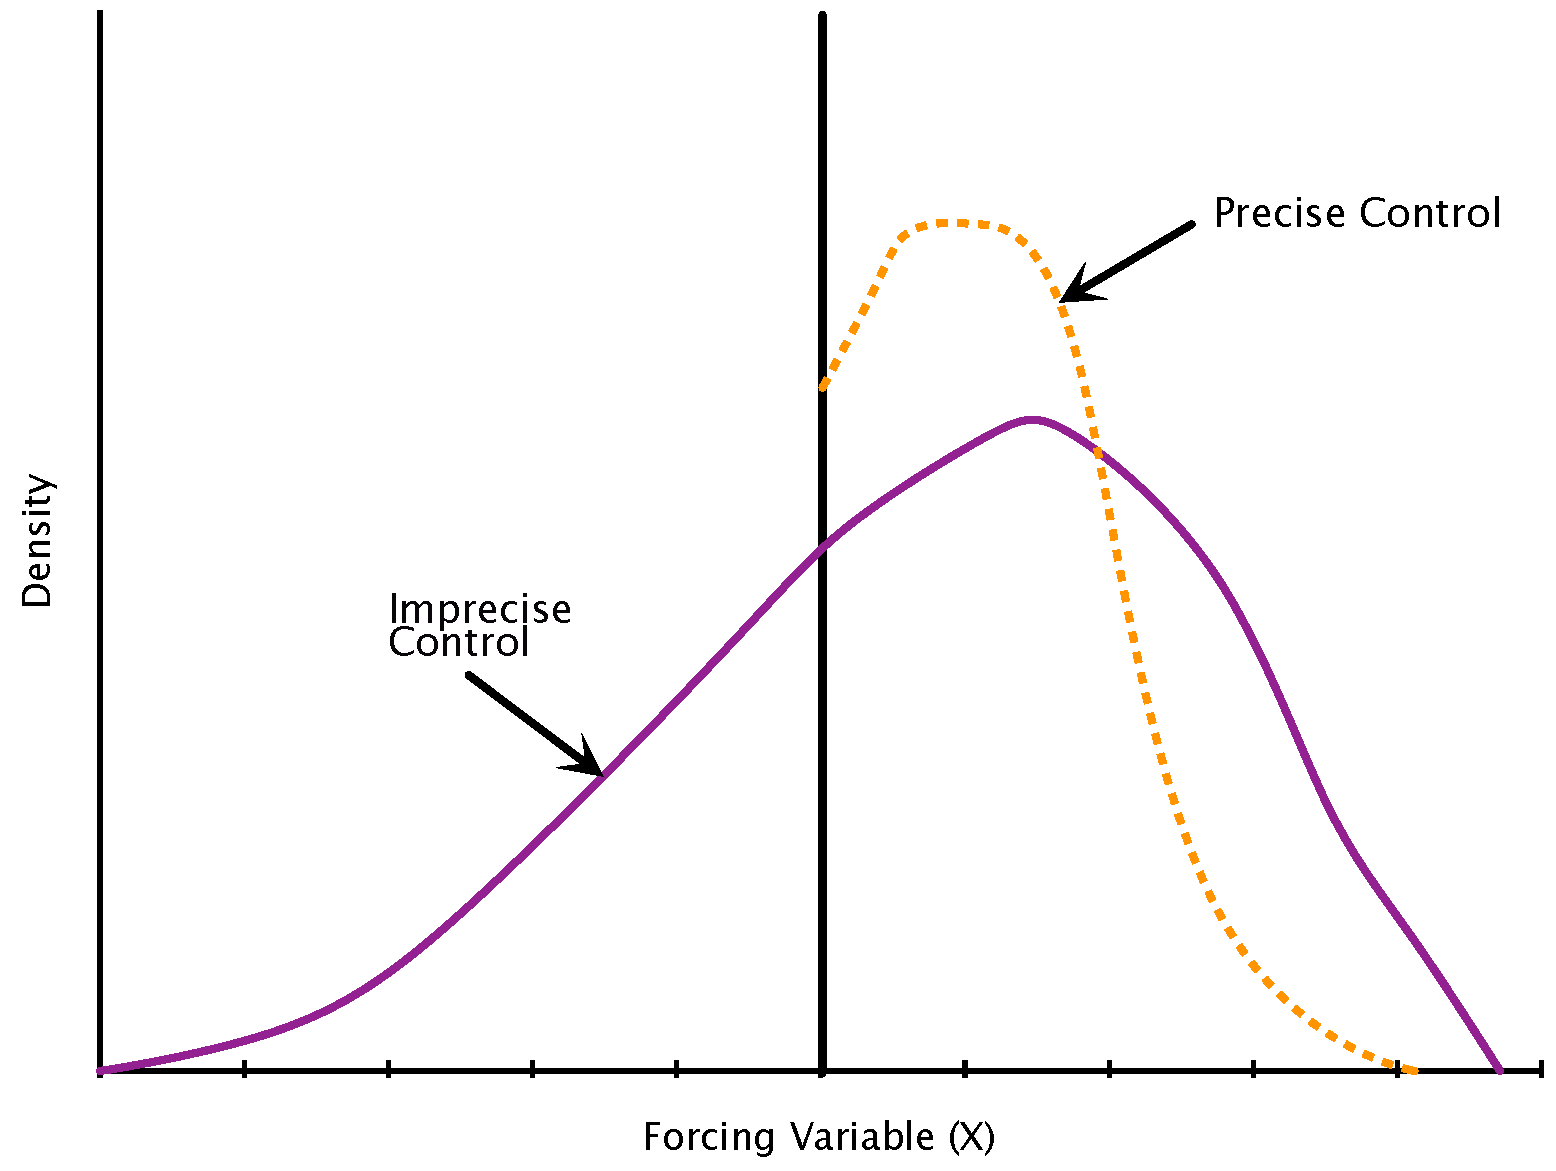
\includegraphics[width=10.5cm]{forcing_control.pdf}  
\end{frame}

\begin{frame}[c]\frametitle{More Lee}
	\begin{itemize}
		\item<+-> \textbf{Definition:} We say individuals have imprecise control over $X$ when conditional on $W=w$ and $U=u$, the density of $V$ (and hence $X$) is continuous.
		\item<+-> \textbf{Local Randomization:} If individuals have imprecise control over $X$ as defined above, then $P(W=w,U=u|X=x)$ is continuous in $x$; the treatment is ``as good as'' randomly assigned around the cutoff. 
	\end{itemize}
\end{frame}

\section{Examples}

\begin{frame}
  \frametitle{Eggers (2009)}  

Duverger's Law (1972): 
\begin{quote}
  To these socio-economic and historical factors a technical factor must be added: the electoral system. I expressed its effects in 1946 in the formulation of three sociological laws: (1) a majority vote on one ballot is conducive to a two-party system; (2) proportional representation is conducive to a multiparty system; (3) a majority vote on two ballots is conducive to a multiparty system, inclined toward forming coalitions.
\end{quote}

In French municipalities, the electoral rule used to elect the municipal council depends on the city's population: cities with fewer than 3,500 people elect their councils by a form of plurality rule, while those with a population of 3,500 or more use a form of PR. 
\end{frame}

\begin{frame}
  \frametitle{Eggers (2009)}  
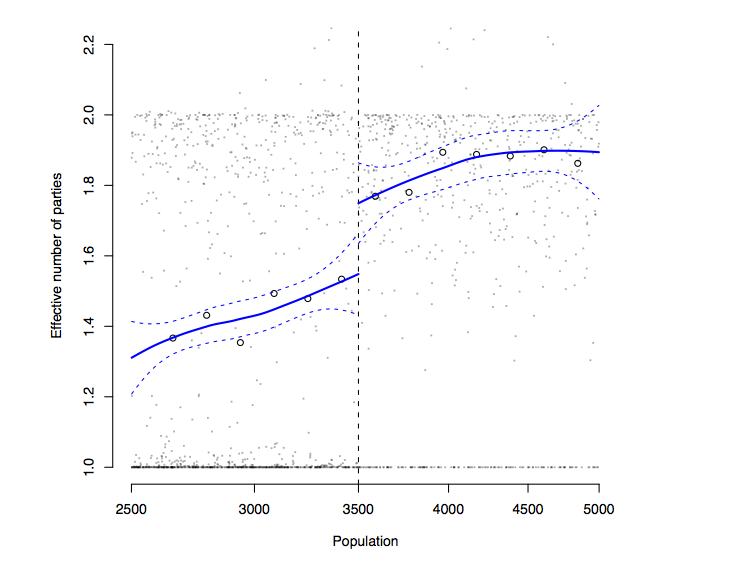
\includegraphics[width=9.5cm]{Eggers.png}  

\end{frame}

\begin{frame}
  \frametitle{Lee and Dinardo (2004)}
Lee and Dinardo document that the outcome of an NLRB election has a
substantial, binding impact on the collective bargaining pro- cess,
even among close elections. Where they barely win the election, unions
are able to maintain their legal recognition over long time horizons;
where they barely lose, there is little evidence of subsequent
attempts to organize the workplace.  

Question: \textbf{What is the impact of union recognition keeping all other things---including having held an elections---equal?}
\end{frame}

\begin{frame}
  \frametitle{Lee and Dinardo (2004)}
Do NLRB elections lead to unionization?
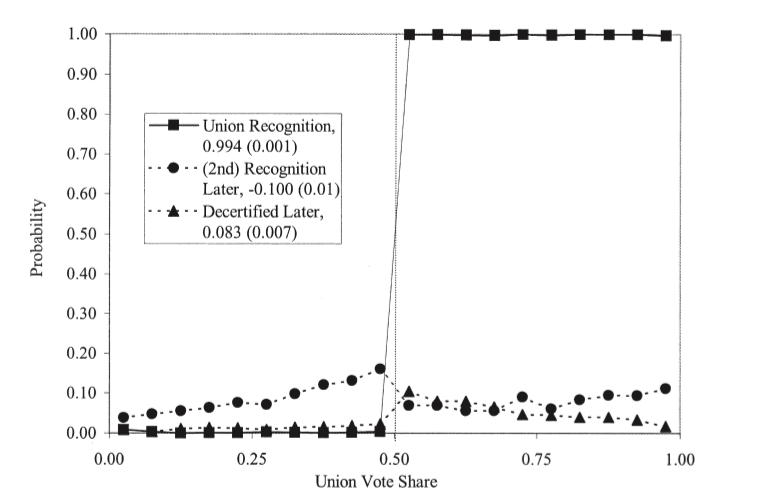
\includegraphics[width=9.5cm]{Lee_Dinardo_Forcing.png}  
\end{frame}

\begin{frame}
Does unionization increase wages?
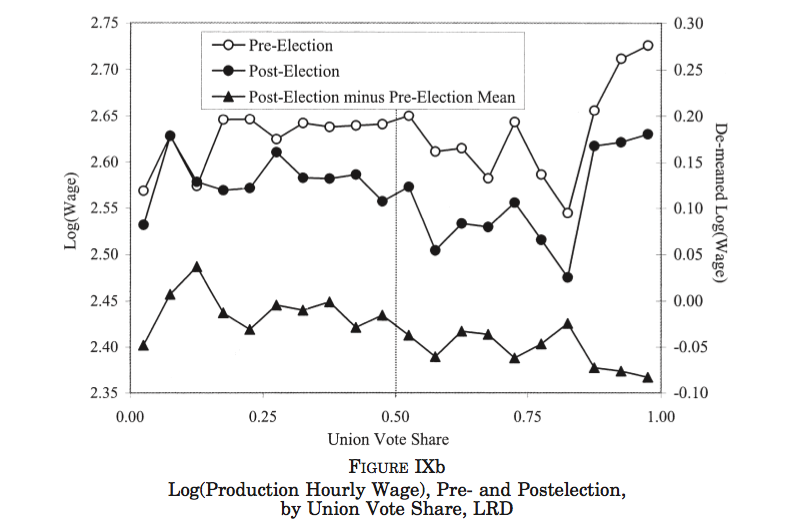
\includegraphics[width=9.5cm]{Lee_Dinardo_Output.png}  

\end{frame}


\begin{frame}
  \frametitle{Dell (2009)}
  \begin{itemize} 
  \item What are the long term impacts of colonial institutions?
  \item Dell (2009) examines the long run impacts of the mining mita, a forced
labor system instituted by the Spanish government in Peru and Bolivia
in 1573 and abolished in 1812. The mita required over 200 indigenous
communities to send one seventh of their adult male population to work
in the Potosi silver and Huancavelica mercury mines
  \item \textit{The contribution of mita conscripts changed discretely at the boundary of the subjected region - on one side all communities sent the same percentage of their population to the mines, while on the other side all communities were exempt}
  \end{itemize}
\end{frame}

\begin{frame}
  \frametitle{Dell (2009)}

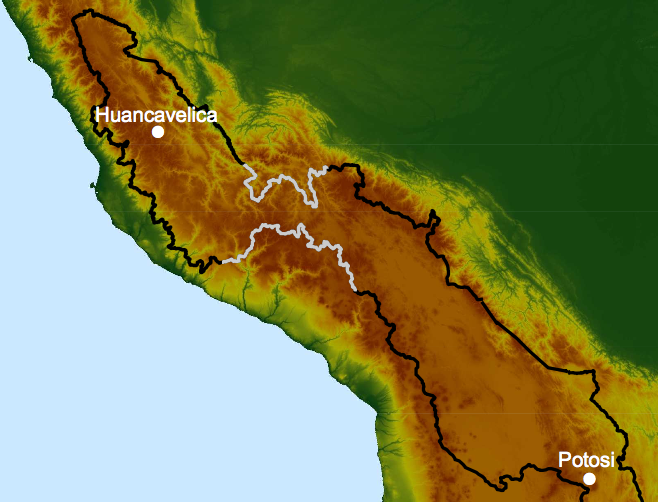
\includegraphics[width=9.5cm]{Mita_boundary.png}  
\end{frame}

\begin{frame}
  \frametitle{Dell (2009)}
The long term impact of the Mita on development outcomes:
  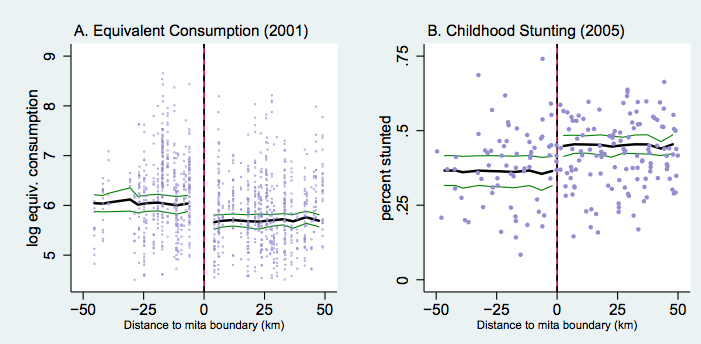
\includegraphics[width=10.5cm]{Mita_results.png}  
\end{frame}

\begin{frame}[c]\frametitle{Urquiola}
	\begin{itemize}
		\item<+-> Chiliean private schools cannot enroll more than 45 students per classroom.
		\item<+->  
		\begin{quote}
			\dots in the presence of the class-size cap and the integer constraint on the number of classrooms, schools at the cap adjust price (or enrollment) to avoid having an additional classroom. This results in stacking at enrollment levels that are multiples of 45. Because higher income households sort into higher-productivity schools, the stacking implies discontinuous changes in average family income and hence in other correlates of income, such as mothers' schooling, at these multiples.
		\end{quote}
	\end{itemize}
\end{frame}

\begin{frame}[t]\frametitle{Urquiola}
	\begin{figure}[htbp]
		\centering
			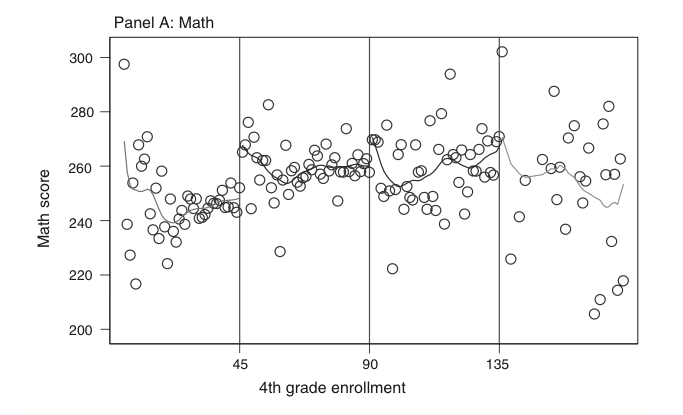
\includegraphics[height=2.5in]{Urquiola1.png}
		\label{fig:Urquiola1}
	\end{figure}
\end{frame}

\begin{frame}[t]\frametitle{Urquiola}
	\begin{figure}[htbp]
		\centering
			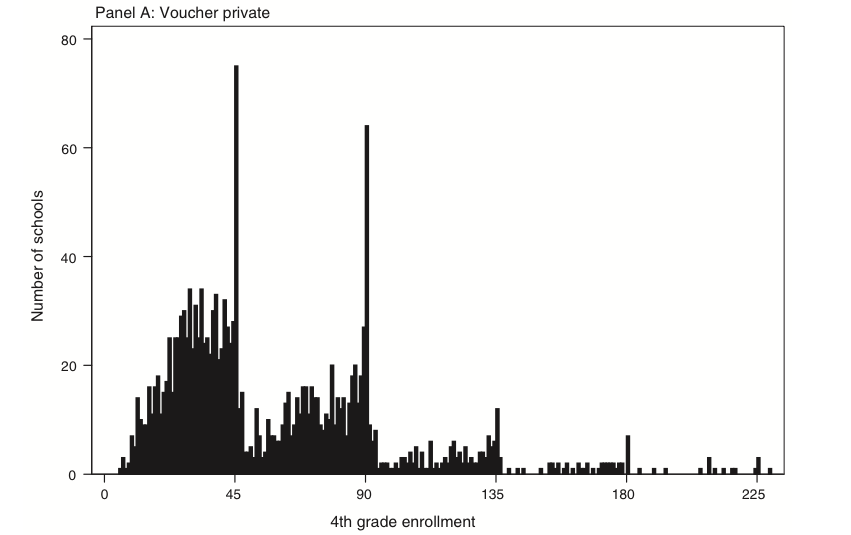
\includegraphics[height=2.5in]{Urquiola2.png}
	\end{figure}
\end{frame}

\begin{frame}[t]\frametitle{Urquiola}
	\begin{figure}[htbp]
		\centering
			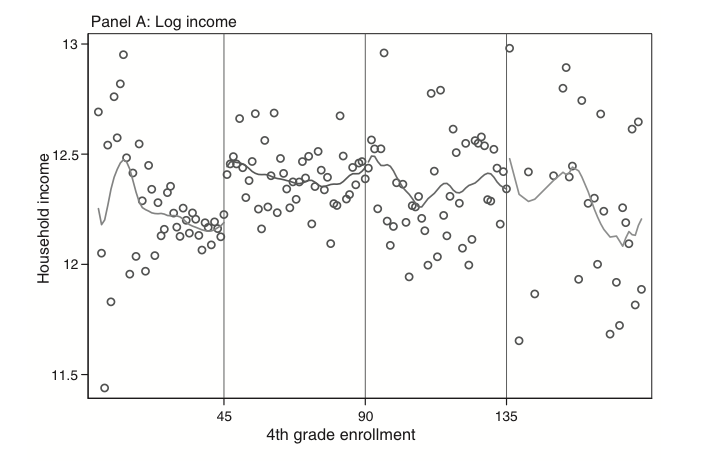
\includegraphics[height=2.5in]{Urquiola3.png}
	\end{figure}
\end{frame}

\section{Nuts and Bolts}

\begin{frame}
  \frametitle{Incumbency (Dis) Advantage in Brazil}
  \begin{itemize}
  \item  Data used in R. Titiunik, ``Incumbency Advantage in Brazil:
    Evidence from Municipal Mayor Elections''
 \item Let municipality $i$ at election $t$ have $J$ political parties
   that dispute municipal mayor elections.
 \item Let $V_{itj}$ be the vote share obtained by party $j$ in
   municipality $i$ in election $t$. 
 \item The margin of victory (or loss) for party $k$ (our forcing variable) is
   defined as $Z_{itk}=V_{itk}-V_{itj}$, where $V_{itj}$ is the vote share of
  party $k$'s strongest opponent. 
\item The rule determining incumbency status:  
\[ T_{it+1,k} = \left\{ 
\begin{array}{l l}
  1 & \quad \mbox{if $Z_{itk} \geq 0$} \\
  0 & \quad \mbox{if  $Z_{itk} < 0$} \\
\end{array}
 \right. \]
\end{itemize}

\end{frame}

\begin{frame}
  \frametitle{Density of the Forcing Variable}
Is there evidence of manipulation?  No. 
  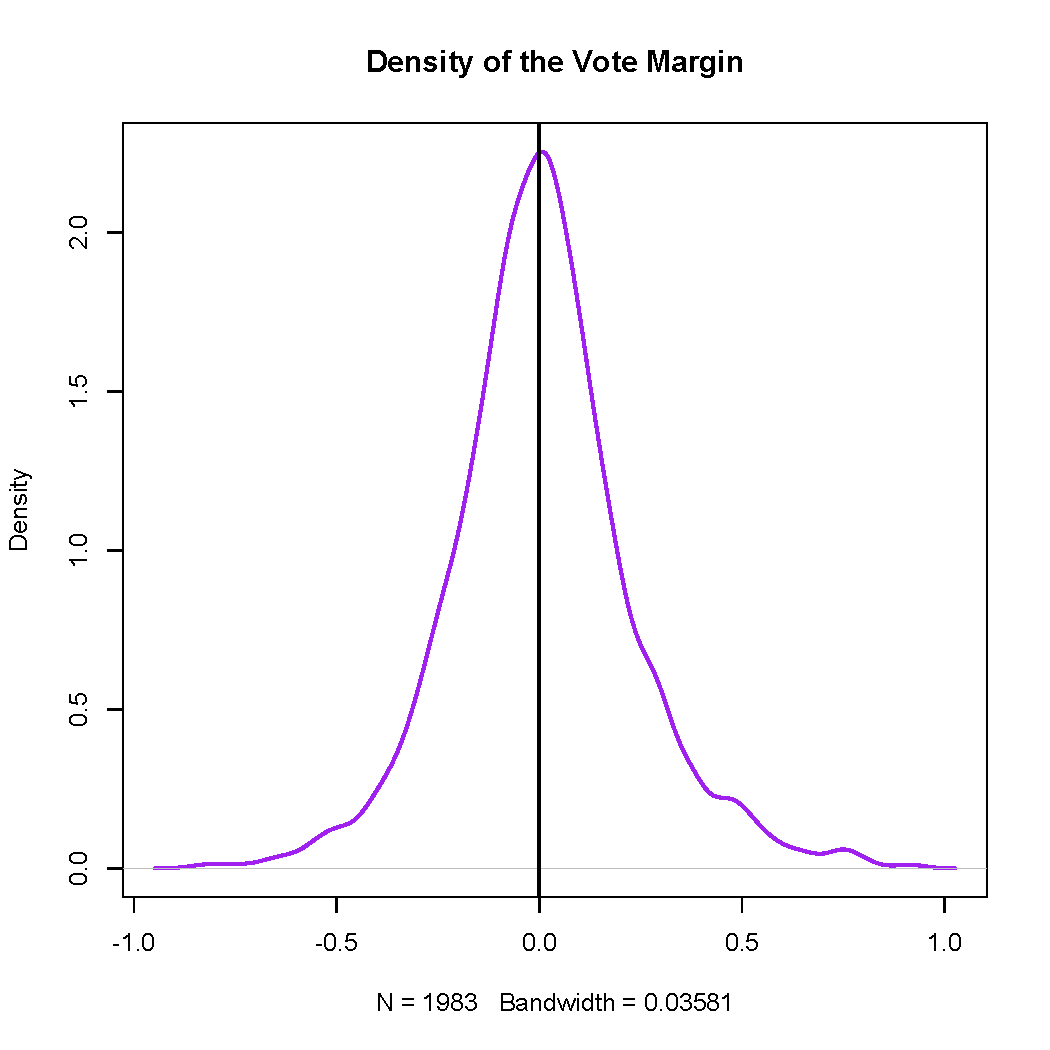
\includegraphics[width=8.5cm]{forcingvar_density.pdf}  
\end{frame}

\subsection{Graphical Methods}
\begin{frame}
  \frametitle{Binning}
  \begin{itemize}
  \item A standard way of graphing the data is to divide the forcing
    variable into a number of bins and then averaging the outcome
    variable in each bin. The bin averages are then plotted against
    the bin mid-points.
  \item The key question is whether there is evidence of a jump in the
    conditional mean of the outcome at the cutoff. If there is no
    visual evidence of a ``jump'' at $c$, it is unlikely that
    more sophisticated analyses will lead to credible effect
    estimates that are different from 0.  More formal 
    analyses are essentially more sophisticated versions of this
    binning procedure.
  \end{itemize}

\end{frame}

\begin{frame}
  \frametitle{Binning}
Using Pre-Treatment Covariates to check the validity of the design:

  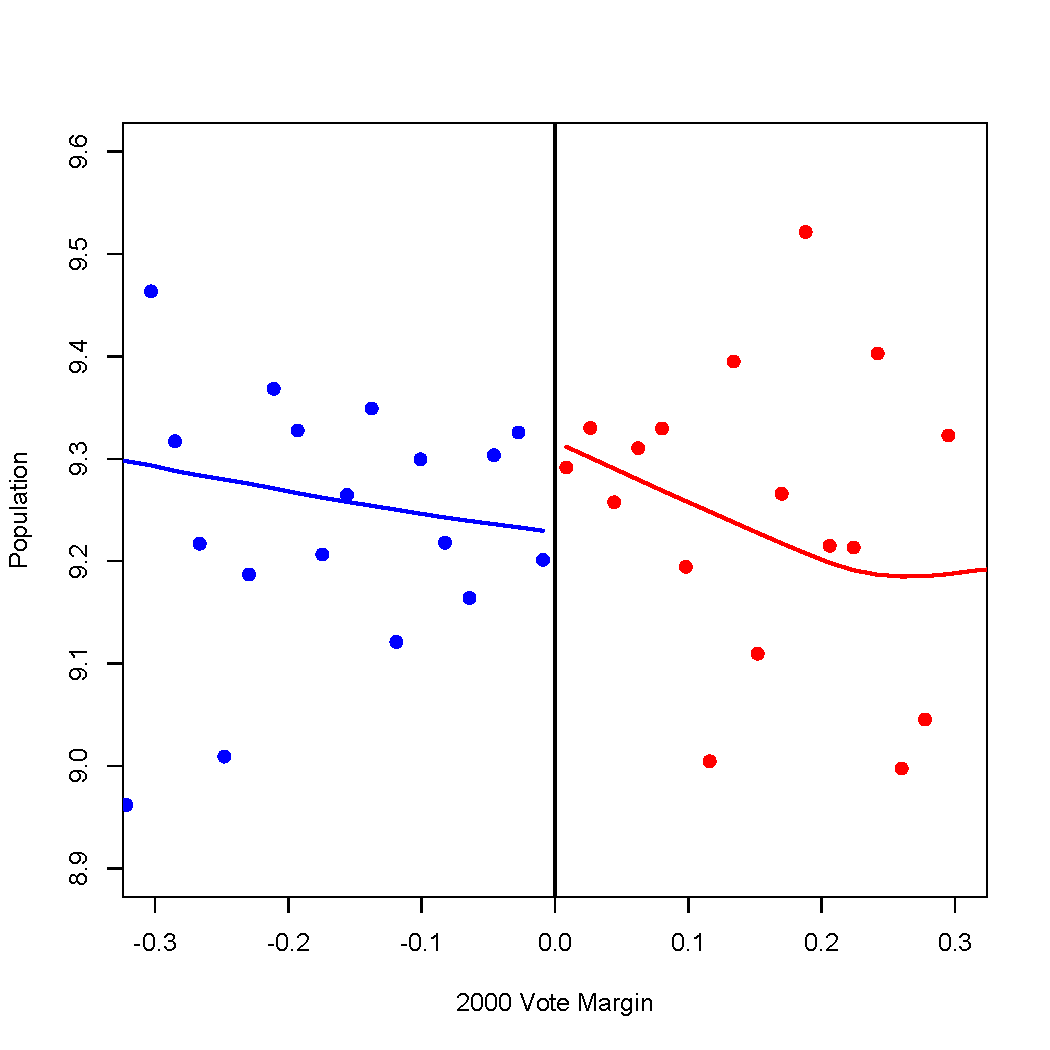
\includegraphics[width=7.5cm]{population_bal_check.pdf}  

\end{frame}

\begin{frame}
  \frametitle{Outcome}
Is there an incumbency advantage? 
  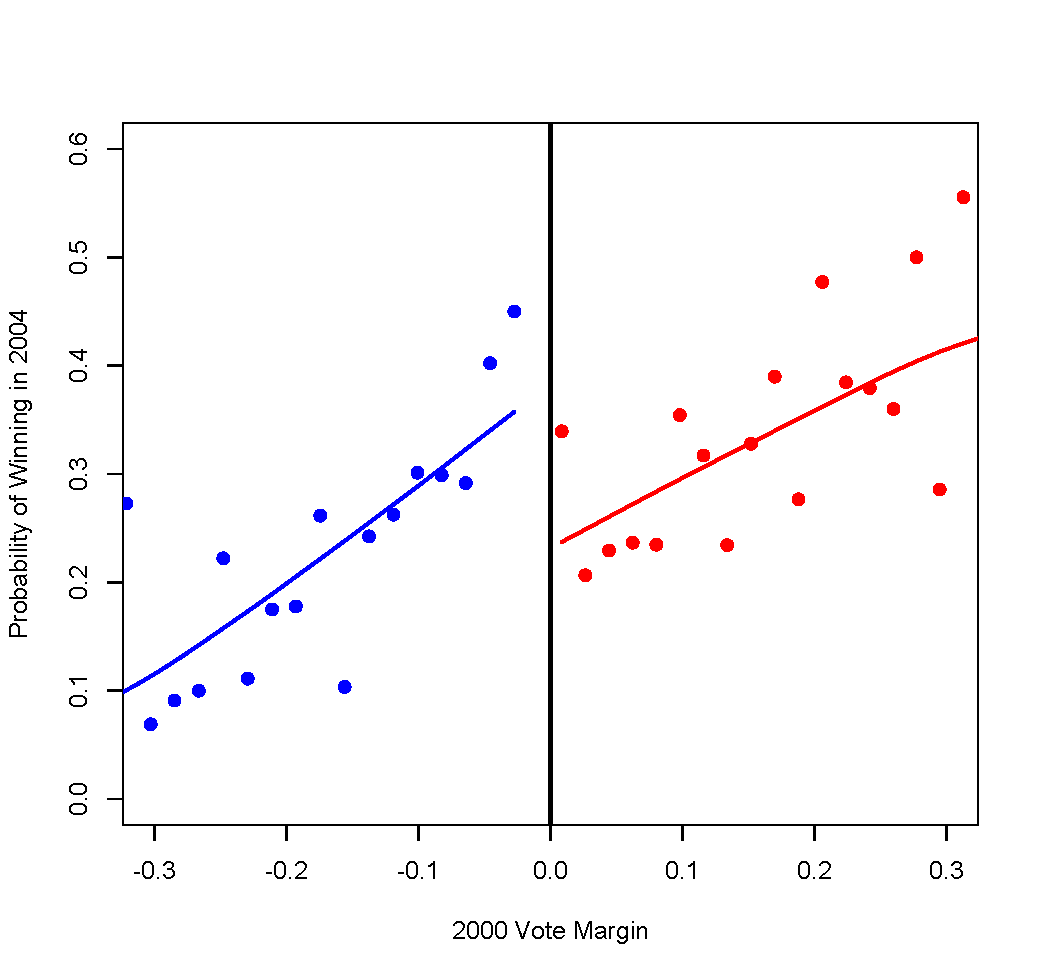
\includegraphics[width=7.5cm]{PMDB_treat_effect.pdf}  

\end{frame}

\subsection{Analysis}
\begin{frame}
  \frametitle{Kernel Estimator}
  \begin{itemize}
  \item Define the conditional means: $\mu_l=E[Y(0)|X=c]$ and $\mu_r=E[Y(1)|X=c]$
  \item The estimand is $\tau_{rd}=\mu_r(c) - \mu_l(c)$.
  \item One approach is to use a kernel $K(u)$, with $\int \! K(u) \,
    du = 1$ and a bandidth of $h$, i.e. your ``window''. 
    \item To calculate $\hat \tau_{RD} = $
$$
\frac{\sum_{i:X_i \geq c} Y_i \cdot K((X_i
  -x)/h)}{\sum_{i:X_i\geq c} K((X_i - x)/h)} - \frac{\sum_{i:X_i < c} Y_i \cdot K((X_i
   -x)/h)}{\sum_{i:X_i< c} K((X_i - x)/h)}
$$
 \end{itemize}
\end{frame}

\begin{frame}
  \frametitle{Rectangular Kernel}
  \begin{itemize}
  \item One common estimator uses a rectangular kernel, which weights each observation in the bandwidth window  equally:
\small
$$
\frac{\sum_{i:X_i \geq c} Y_i \cdot 1\{c\leq X_i \leq c + h\}}{1\{c\leq X_i \leq c + h\}} - \frac{\sum_{i:X_i \geq c} Y_i \cdot 1\{c-h\leq X_i \leq c \}}{1\{c-h\leq X_i \leq c\}}
$$
\normalsize
\item  This estimator can be interpreted as first throwing away observations with a value of $X_i$ more than $h$ away from $c$, and then simply differencing the average outcomes by treatment status in the remaining sample. 
\end{itemize}
\end{frame}

\begin{frame}
  \frametitle{Rectangular Kernel}
  \begin{itemize}
  \item One common estimator uses a rectangular kernel, which weights each observation in the bandwidth window  equally:
\small
$$
\frac{\sum_{i:X_i \geq c} Y_i \cdot 1\{c\leq X_i \leq c + h\}}{1\{c\leq X_i \leq c + h\}} - \frac{\sum_{i:X_i \geq c} Y_i \cdot 1\{c-h\leq X_i \leq c \}}{1\{c-h\leq X_i \leq c\}}
$$
\normalsize
\item  This estimator can be interpreted as first throwing away observations with a value of $X_i$ more than $h$ away from $c$, and then simply differencing the average outcomes by treatment status in the remaining sample. 
\end{itemize}
\end{frame}

\begin{frame}
  \frametitle{Local Linear Regression}
  \begin{itemize}
  \item Instead of locally fitting a constant function, we can fit linear regression functions to the observations within a distance $h$ on either side of the discontinuity point:
\small
$$
\textrm{min} \sum_{i:c-h<X_i<c} (Y_i-\alpha_l - \beta_l\cdot(X_i-c))^2
$$
and 
$$
\textrm{min} \sum_{i:c \leq X_i<c+h} (Y_i - \alpha_r - \beta_r \cdot(X_i-c))^2
$$

\normalsize
\item The value of $\mu_l(c)$ is estimated as $\hat \mu_l(c)= \hat \alpha_l + \hat \beta_l \cdot (c-c)=\hat\alpha_l$ and  $ \hat \mu_r(c)$ is estimated as $\hat \mu_r(c)= \hat \alpha_l + \hat \beta_l \cdot (c-c)=\hat\alpha_r$.
\item $\hat \tau_{RD} = \hat \alpha_r - \hat \alpha_l$.
\end{itemize}
\end{frame}

\section{Cross-Validation}

\frame{
	\frametitle{Cross-Validation}
        \begin{itemize}
          \item How do we check the accuracy of a predictive model? 
        \item  Many predictive models tend to over-fit, so  good
          practice is to choose a predictive model based on a  training data set and then check its predictive accuracy on a seperate validation dataset.
          \item Training datasets aren't available, as in our regression discontinuity
case, but one useful technique for testing our model's predictive
accuracy is known as \textbf{cross-validation}. 
        \end{itemize}
}

\frame{
	\frametitle{Cross-Validation}
        \begin{itemize}
          \item We usually refer to prediction error as the expected squared difference between a future response and its prediction from the model:
$$\textrm{PE}=E\{(y-\hat y)^2 \}$$
          \item In cross validation, we use part of the data to fit the model, and a different part to test it. 
          \item Suppose we split the data into $K$ parts. Let $k(i)$ be the part containing observation $i$. Denote the by $\hat y_i^{-k(i)}$, the fitted value for observation $i$, computed with the $k(i)$th part of the data removed. Then the cross-validation prediction error is:
$$\textrm{CV} = \frac{1}{n} \sum_{i=1}^n(y_i-\hat y_i^{-k(i)})^2$$
        \end{itemize}
}

\frame{
	\frametitle{``Leave-One-Out''}
        \begin{itemize}
          \item Often we choose $k=n$, resulting in \textbf{``leave-one-out''} cross-validation.
          \item For each observation $i$, we refit the model leaving that observation out of the data, and then compute the predicted value for the $i$th observation and compute the predicted value $\hat y_i^{-i}$. We do this for each observation and then compute the average cross-validation sum of squares $\textrm{CV} = \sum (y_i - \hat y_i^{-i})^2/n$
        \end{itemize}
}


\frame{
What are we predicting?

\small
$$
\textrm{min} \sum_{i:c-h<X_i<c} (Y_i-\alpha_l - \beta_l\cdot(X_i-c))^2
$$
and 
$$
\textrm{min} \sum_{i:c \leq X_i<c+h} (Y_i - \alpha_r - \beta_r \cdot(X_i-c))^2
$$

\normalsize
\begin{itemize}
\item The value of $\mu_l(c)$ is estimated as $\hat \mu_l(c)= \hat
  \alpha_l + \hat \beta_l \cdot (c-c)=\hat\alpha_l$ and $ \hat
  \mu_r(c)$ is estimated as $\hat \mu_r(c)= \hat \alpha_r + \hat
  \beta_r \cdot (c-c)=\hat\alpha_r$.
\item $\hat \tau_{RD} = \hat \alpha_r - \hat \alpha_l$.
\end{itemize}
}


\frame{
	\frametitle{Effect of Incumbency on Vote Share}
     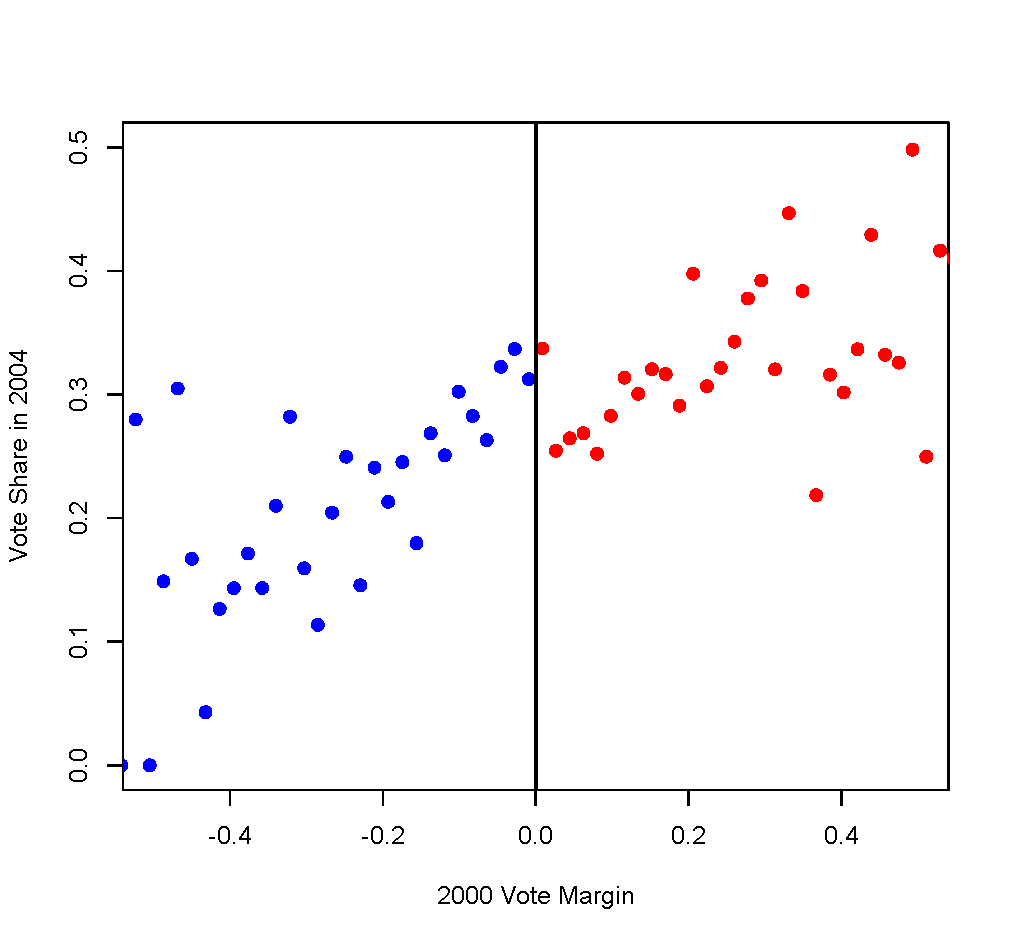
\includegraphics[width=8cm]{vote_share_discont.pdf}  

}

\frame{
\frametitle{Picking \textit{h}}
  \begin{itemize}
  \item We need to pick an $h$ and cross-validation is a natural ``hands-off'' technique. 
  \item Predict each $y_i$ using $x_i$ values within $h$. Note that we each treat each $y_i$ as point at a boundary.
  \item To emulate the fact that RD estimates are based on regression estimates at the boundary,
the regression is estimated using only observations with values of $X$
on the left of $X_i$ ($X_i-h \leq X <X_i$) for observations on the
left of the cutpoint ($X_i<c$). For observations on the right of the
cutoff point ($X_i\geq c$), the regression is estimated using only the
observations with values of $X$ on the right of $X_i$ ($X_i<X\leq
X_i+h$)

  \end{itemize}
}

\frame{
  \begin{itemize}
  \item Formally, let $\hat Y(X_i)$ be the predicted value of $Y$ obtained
using the regressions described above. The cross validation criterion
is defined as
$$
\textrm{CV}_Y(h) = \frac{1}{N}\sum_{i=1}^N(Y_i-\hat Y(X_i))^2
$$
with the corresponding cross-validation choice for the bandwidth
$$
h_{\textrm{CV}}^{\textrm{opt}} = \arg \min_h \textrm{CV}_Y(h)
$$

  \end{itemize}
}

\frame{
	\frametitle{Results of Cross-Validation}
     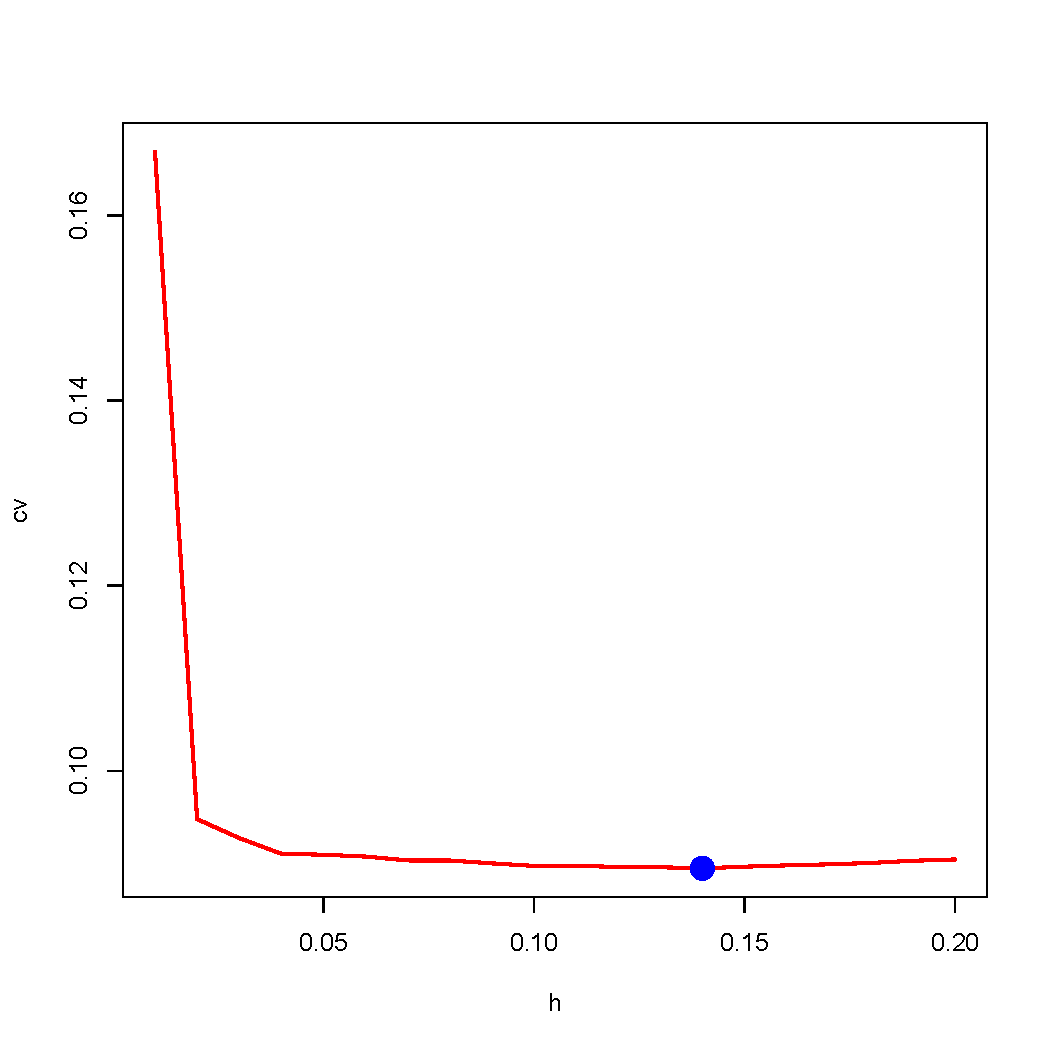
\includegraphics[width=8cm]{cross_valid.pdf}  

}


   

\end{document}
